% ##################################################################################################################
\chapter{London}
\label{ch:london}
\hfill \textbf{Authors:} Joan Serras, Melanie Bosredon, Vassilis Zachariadis, Camilo Vargas-Ruiz, Thibaut Dubernet, Mike Batty

\editdone{This text has undergone the professional edit. Please no grammatical changes anymore! They are most-probably wrong.}

% ##################################################################################################################
The building of a London travel demand model began with the EUNOIA Project.%
\footnote{see \url{http://eunoia-project.eu}} 
Core model design decisions were made after two meetings with \gls{tfl}, part of the project Advisory Board; 
\gls{tfl}'s main suggestion was the adaption of an activity-based approach.

Main features of the current London model implementation were:
%
\begin{itemize}\styleItemize
\item     Baseline year was 2010.
\item	Geographic case study area extent was bounded by the M25 and included about 9,4\,million inhabitants (Census~2011)
\item	Types of activity in the model were: home, work, shop, education, leisure and other.
\item	Four travel modes were included: walk, cycle, car and public transport. Public transport mode included buses, underground, rail, Docklands Light Railway and the London Overground.
\item	 London model analysis zones were the English Census~2011 Wards, referred to as wards; our case study was composed of 850\,wards.
\end{itemize}
%
% ##################################################################################################################
\section{Supply}
The supply assembly for our model defined these three components:
%
\begin{itemize}\styleItemize
\item	Road network
\item	Public transport services
\item	Land-use configuration
\end{itemize}
%
Integrated Transport Network from the Ordnance Survey provided data used to build the road network. 
The source network, defined at navigation level, was processed to remove some detail. 
Decisions on each road link's capacity was based on guidelines proposed by the COBA Manual~(2002)(Vol.~13),%
\footnote{retrieved from \url{https://www.gov.uk/government/publications/coba-11-user-manual}} 
by the UK’s Department for Transport. 
This involved usage of each road link’s road type (Motorway or A road, etc.) and road nature (single carriageway, dual carriageway or slip road, among others) to establish road capacity for each link.

Information on all case study region public transport services was obtained from National Public Transport Data Repository from~2009%
\footnote{see \url{http://data.gov.uk/dataset/nptdr}} timetable data; this dataset included a very detailed account of all UK services.

Finally, land-use configuration for the London model was produced using the Ordnance Survey \lstinline|AddressBase| layer that held address records for the whole United Kingdom, with individual land-use definitions. 
We processed detailed spatial information to assign each address point to the nearest network road link; after this process, each link in our network contained many addresses with associated land use. 
We also mapped multiple categorizations attached to each address point with model activity types: home, work, shop, education, leisure and other.

% ##################################################################################################################
\section{Demand}
To define travel demand associated with London, we followed methodology adopted in \gls{transims}%
\footnote {We used v3.1, corresponding to that developed in Los Alamos National Laboratory.}. We first generated a synthetic population representative of the case study area and then assigned each synthetic individual a sequence of activities.

We created our synthetic population using a simulated annealing technique based on \citet[][]{metropolissampling}, using the following two datasets: Census~2011 data for each of the 850\,wards in London and the \gls{hsar} for England in~2001. This technique was based on a survey household selection from the \gls{hsar}, that best matched overall socio-demographics from the Census~2011 for each of the 850\,wards in London. This technique output included a number of synthetic households associated with each ward and, correspondingly, synthetic individuals living in the household, with very detailed socio-demographic information.

Each synthetic household was assigned to our network using a probabilistic distribution based on the use of home-only activity locations within each ward.

Skeletal activity pattern assignment for each synthetic individual was executed using Classification and Regression Tree Algorithms similar to \citet[][]{SpeckmanEtAl_TechRep_NISS_1998}: specifically, the multivariate regression tree algorithm. 
This technique aimed to produce clusters of survey households with similar activity patterns through the use of socio-demographic data. 
Once the decision tree was built, it was used to assign each synthetic household to a given survey household through socio-demographic similarities between the two. 
In this case study, we used the \gls{ltds}~2010/11 to generate the tree.

After assigning skeletal activity patterns to each synthetic individual, we next assigned each activity a location. 
To do this, we used a multinomial logit choice model. This technique allowed each synthetic individual to evaluate the benefit of performing a specific activity at a particular destination as a composite value, based on objective metrics associated with the destination (\eg number of relevant addresses), objective metrics associated with traveling from origin to destination (\eg travel time) and subjective components following a probability distribution. Wards, again, made up the area units considered in London; each ward's attractiveness was quantified by number of addresses for each activity type and accessibility throughout the region (travel time across all wards using crow-fly distances and average speed for each travel mode). Each travel mode and activity type pair was calibrated and those parameters were used to calculate new activity locations for each synthetic agent.

% ##################################################################################################################
\section{Calibration and Validation}
For calibration, the multinomial logit choice model applied described in the previous section could also have been included here and activity-related time values were set in \gls{matsim}’s configuration file, using typical duration values observed from the \gls{ltds} dataset. 
Finally, parameter values set by default in \gls{matsim} 
%taking the Vickrey scenario values 
were also adopted here. This was a limitation, as the modal split then in place was that provided by the \gls{matsim} corresponding module. 
Related parameters should first be adjusted, so that observed modal share is similar across modes.

For validation, traffic counts from approximately 600\,sensors were made available to us for London. We held values for the morning peak (8-9\,am), the inter-peak (9\,am-5\,pm) and the evening peak (5-6\,pm). The former and the latter were hourly counts; the inter-peak was an average value. 
Those counts were organised into so-called cordons (3) and screenlines (3). Comparisons are currently taking place; we are not yet in a position to evaluate, in detai,l how the model validated with the data observed.

% ##################################################################################################################
\section{More Information}
More detailed information on the building of the model, including some results from each module previously 
described, can be found at: \url{http://eunoia-project.eu/publications/} (Report on Case Study~1: London).

% ##################################################################################################################
 % ------------
\createfigure%
{Snapshot of the road network for London's case study}%
{Snapshot of the road network for London's case study colored by road type (left) and map showing number of bus trips per road segment in London using timetable data (right)}%
{\label{fig:london_fig1}}%
{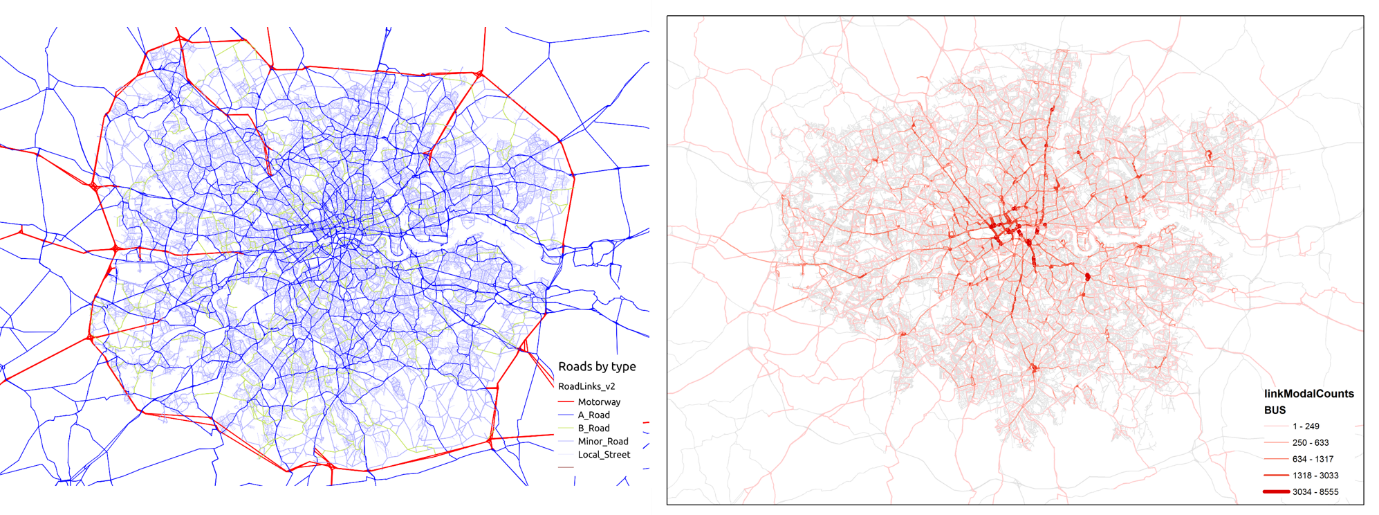
\includegraphics[width=0.95\textwidth, angle=0]{scenarios/figures/london1.png}}%
{}
% ------------
 % ------------
\createfigure%
{Visual estimate of activities performed in London at 9am using the \gls{via} software}%
{Visual estimate of activities performed in London at 9\,am using the \gls{via} software}%
{\label{fig:london_fig2}}%
{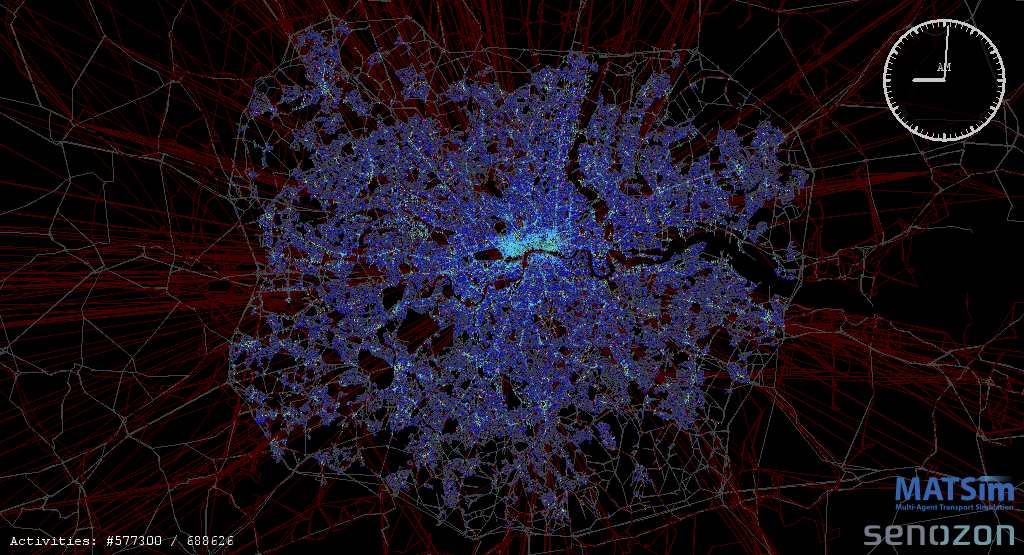
\includegraphics[width=0.95\textwidth, angle=0]{scenarios/figures/london2.png}}%
{}
% ------------

% ##################################################################################################################










